\subsection{Large scale simulations}
\label{sec:largescale}


In order to verify that the designed methods can also work in realistic Internet-like topologies, we 
performed large-scale simulations using a modified version of Rocketfuel AT\&T topology~\cite{rocketfuel}.
To approximate structure of the Internet, we selected the largest connected component of 562 nodes and separated nodes in three categories: clients, gateways, and backbones.
All nodes with degrees one, two, and three became clients (344 red nodes on Fig.~\ref{fig:large-scale}), all nodes that are directly connected to clients became gateways (109 green nodes), and the rest became backbones (109 blue nodes).
(To ensure that paths in the topology are ``valley-free,'' we augmented the topology with necessary backbone-to-backbone links.)
After categorizing the nodes, we randomly assigned bandwidths and link delays based on link types (see Table~\ref{tab:large-scale}).

\begin{figure}[htbp]
  \centering
  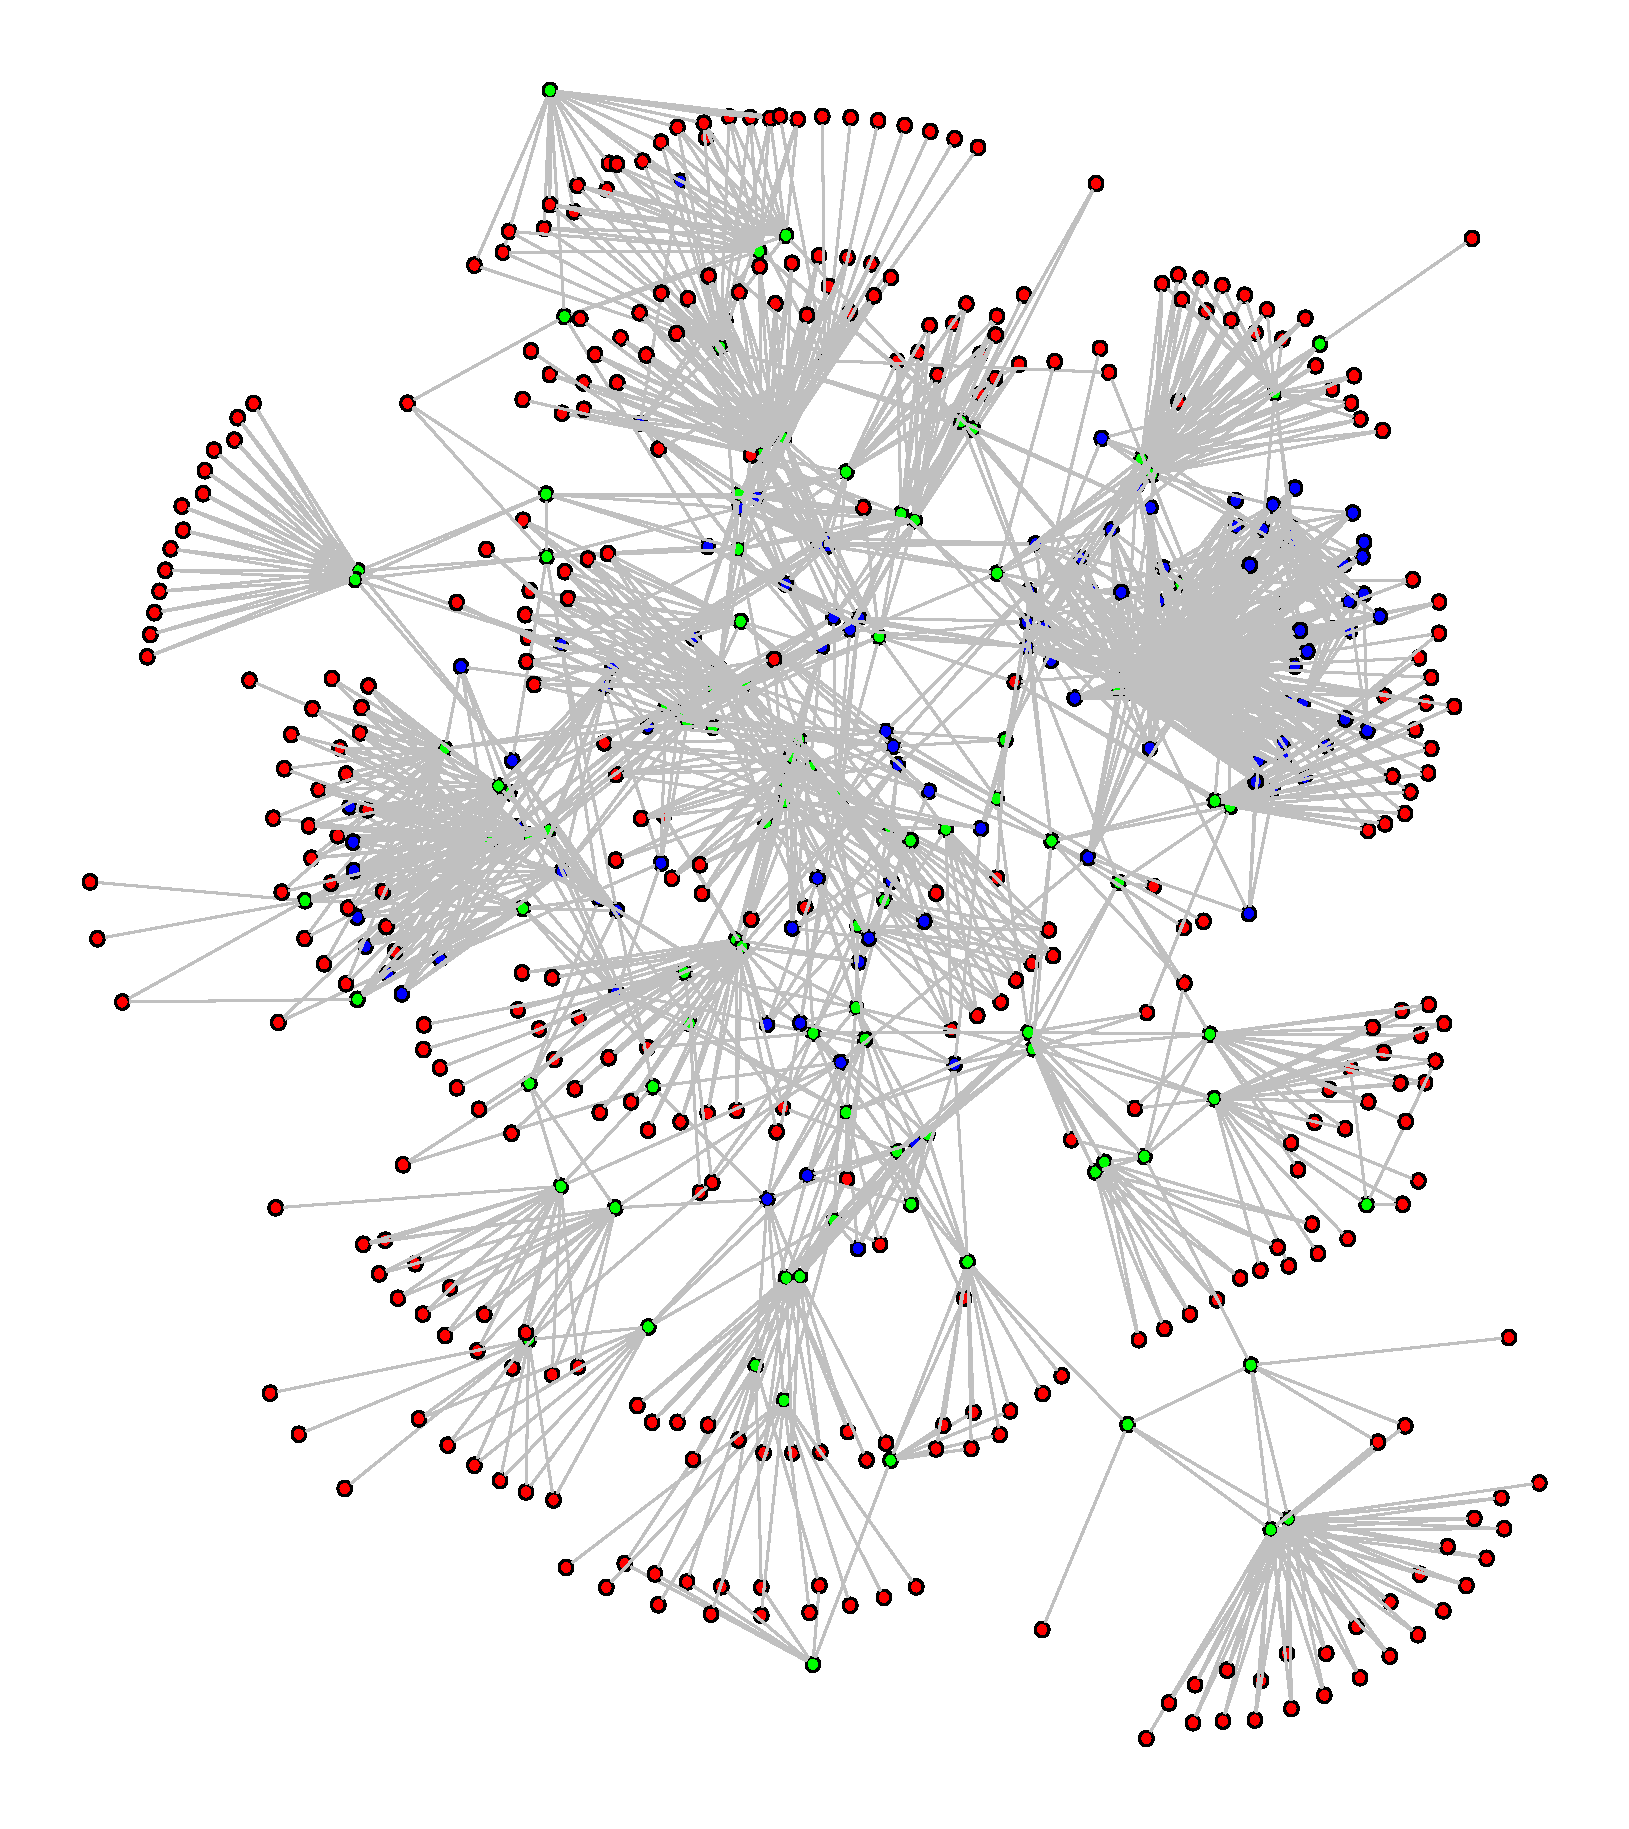
\includegraphics[scale=0.26,angle=90]{7018-r0}
  \caption{Internet-like topology: 344 client routers (red), 109 gateway routers (green), 109 backbone routers (blue)}
  \label{fig:large-scale-topo}
\end{figure}


\begin{table}[htbp]
\centering
\caption{Large-scale topology parameters}
\label{tab:large-scale}
\begin{tabular}{|l||c|c||c|c|}
  \hline
  \multirow{2}{*}{\bf Link type} &  \multicolumn{2}{|c||}{\bf Delay} &  \multicolumn{2}{|c|}{\bf Bandwidth} \tabularnewline
  \cline{2-5}
                        &  Min & Max                       &  Min & Max \tabularnewline
  \hline \hline
  Backbone--Backbone    & 5~ms & 10~ms   & 40~Mbps & 100~Mbps \tabularnewline
  \hline
  Gateway--Backbone,    & \multirow{2}{*}{5~ms} & \multirow{2}{*}{10~ms}   
                        & \multirow{2}{*}{10~Mbps} & \multirow{2}{*}{20~Mbps} \tabularnewline
  Gateway--Gateway      & & & & \\
  \hline
  Client--Gateway       & 10~ms & 70~ms   & 1~Mbps  & 3~Mbps \\
  \hline

\end{tabular}
\end{table}


\begin{figure*}[t]
 \centering
 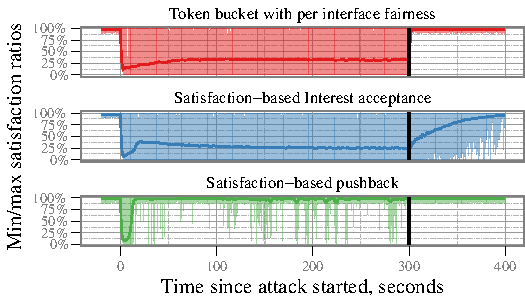
\includegraphics[scale=1]{topo-7018-gw-15mins-new/7018-r0-good-0-producer-gw}
 \caption{Satisfaction ratio dynamics during the attack (30\% attackers)}
 % producer on a gateway node
 \label{fig:large-scale}
\end{figure*}


% \begin{figure*}[t]
%  \centering
%  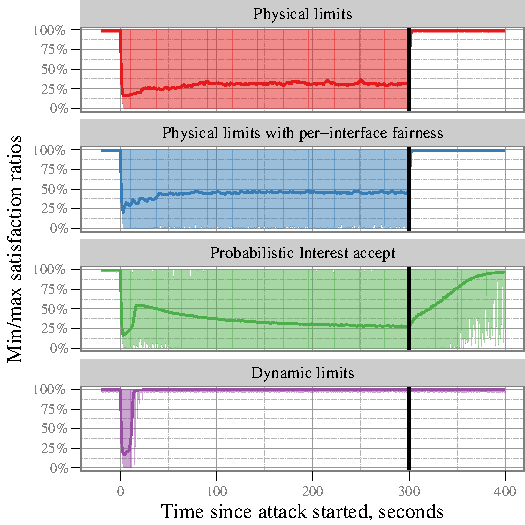
\includegraphics[scale=1]{topo-7018-bb-15mins-new/7018-r0-good-0-producer-bb}
%  \caption{Satisfaction ratio dynamics during the attack (30\% attackers)}
%  % producer on a backbone node
%  \label{fig:large-scale}
% \end{figure*}


%%% Local Variables: 
%%% mode: latex
%%% TeX-master: "paper"
%%% End: 
